Este cap\'{i}tulo describe el proceso seguido para la generaci\'{o}n del modelo de detecci\'{o}n de anomal\'{i}as de manejo. Seg\'{u}n lo repasado en el cap\'{i}tulo anterior, en el presente trabajo, se propone un m\'{e}todo de detecci\'{o}n de anomal\'{i}as de conducci\'{o}n siguiendo un enfoque semi-supervisado, el cual consta de dos componentes: un \textbf{modelo ajustado al comportamiento normal de manejo de un agente} y un \textbf{m\'{e}todo de umbral para detecci\'{o}n de valores at\'{i}picos}. 

\section{Conjunto de muestra}

En el Cap\'{i}tulo 3 se describi\'{o} el proceso de captura y preparaci\'{o}n del conjunto de datos, as\'{i} como tambi\'{e}n su divisi\'{o}n en conjunto de entrenamiento/desarrollo/prueba; sin embargo cabe aclarar que en este cap\'{i}tulo s\'{o}lo se enfoc\'{o} en el  \textbf{conjunto de datos normales}, los cuales corresponden a aquellos datos que no cuentan con una etiqueta; por lo que es el conjunto que se usa para entrenar el modelo que se ajusta al comportamiento normal de manejo.

\vspace{5mm} %5mm vertical space

A pesar de contar con una gran cantidad de datos normales se debe recolectar datos que correspondan a anomal\'{i}as con el objetivo de poder validar el m\'{e}todo de umbral para la detecci\'{o}n de anomal\'{i}as que se propone en este proyecto. Por lo que se debi\'{o} proceder a la captura de  \textbf{datos an\'{o}malos}, el cual est\'{a} conformado seg\'{u}n el Cuadro \ref{table:conjunto_anomalias}.

\begin{table}[]
\centering
\begin{tabular}{|l|l|l|}
\hline
Tipo de anomal\'{i}a & Nro anomal\'{i}as & Nro de datos \\ \hline
Frenos en seco    & 15  & 100  \\ \hline
Giros a la derecha e izquierda a alta velocidad & 15  & 450  \\ \hline
Giros en U a alta velocidad & 100 & 300 \\ \hline
\end{tabular}
\caption{Tabla del conjunto de anomal\'{i}as.}
\label{table:conjunto_anomalias}
\end{table}

\vspace{5mm} %5mm vertical space

Como se mencion\'{o} en el anterior p\'{a}rrafo el conjunto de anomal\'{i}as fue capturado para validar el m\'{e}todo de umbral para la detecci\'{o}n de anomal\'{i}as, por lo que este conjunto ser\'{a} etiquetado como positivo (con la etiqueta 1) y el conjunto de datos normales ser\'{a}n etiquetados como muestras negativas (con la etiqueta 0).

\section{Modelo de detecci\'{o}n de anomal\'{i}as}

\subsection{Generaci\'{o}n de series temporales}

Para la generaci\'{o}n del modelo de detecci\'{o}n de anomal\'{i}as se opt\'{o} por algoritmos de aprendizaje autom\'{a}tico enfocados en series de tiempo, dado que los datos, de los sensores capturados por el dispositivo m\'{o}vil, dependen del tiempo en el que fueron capturados; por lo cual el primer paso a realizar es la generacion de peque\~{n}as fracciones de series temporales, esto permitir\'{a} que el modelo propuesto vaya m\'{a}s all\'{a} de una simple detecci\'{o}n de anomal\'{i}as puntuales y pueda detectar anomal\'{i}as contextuales o colectivas.

\vspace{5mm} %5mm vertical space

En el Cuadro \ref{table:series-de-tiempo} se presenta los resultados de diferentes tama\~{n}os de series de tiempo, observando esos resultados en primera instancia se descarta la serie de tiempo que cuenta con s\'{o}lo un paso en el tiempo debido a que su uso se limitar\'{i}a a una mera detecci\'{o}n de anomal\'{i}as puntuales, lo cual no es el objetivo del presente trabajo de grado, por otra parte la serie temporal que tiene dos pasos no es lo suficientemente descriptiva raz\'{o}n por la que esta serie de tiempo tambi\'{e}n queda descartada, llegando a este punto moment\'{a}neamente no es posible definir la cantidad correcta de pasos en las series de tiempo, por lo cual al igual que la cantidad de componentes principales, ser\'{a} un par\'{a}metro a optimizar en los diferentes experimentos que se realizar\'{a} en las siguientes secciones. Cabe recalcar que el dominio de esta variable estar\'{a} entre 3 a 5 pasos y el de la cantidad de componentes principales estar\'{a} entre 3 y 4.

\begin{landscape}
\pagestyle{empty}
\begin{table}[p!]
\centering
\begin{tabular}{|l|l|l|l|l|l|}
\hline
\multicolumn{1}{|c|}{\multirow{2}{*}{\textbf{\begin{tabular}[c]{@{}c@{}}Nro de \\ Componentes\end{tabular}}}} & \multicolumn{5}{c|}{\textbf{Tama\~{n}os de series de tiempo}}                                                                                                               \\ \cline{2-6} 
\multicolumn{1}{|c|}{}                                                                                        & \multicolumn{1}{c|}{\textbf{1}} & \multicolumn{1}{c|}{\textbf{2}} & \multicolumn{1}{c|}{\textbf{3}} & \multicolumn{1}{c|}{\textbf{4}} & \multicolumn{1}{c|}{\textbf{5}} \\ \hline
3                                                                              & \adj{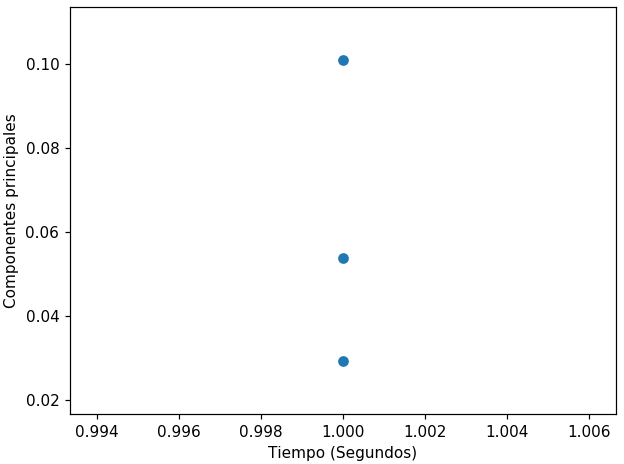
\includegraphics[width=1.5in]{imagenes/Cap4/pca3-1}} &\adj{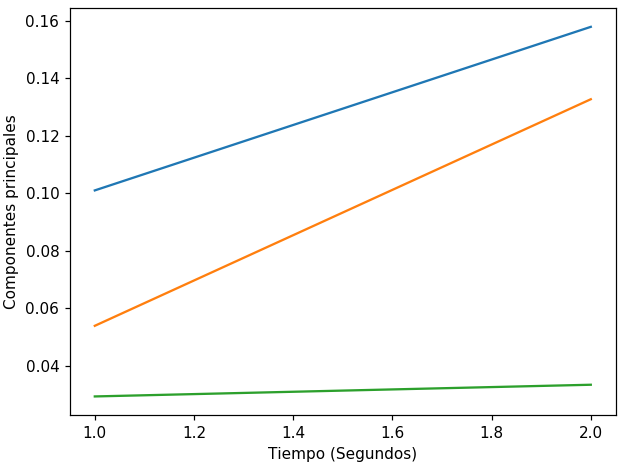
\includegraphics[width=1.5in]{imagenes/Cap4/pca3-2}}&\adj{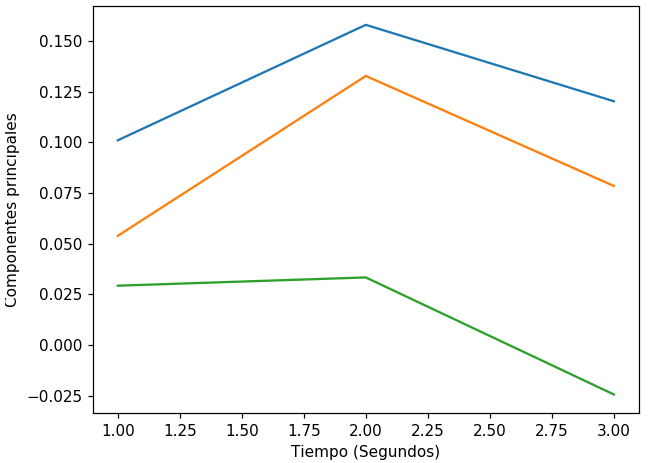
\includegraphics[width=1.5in]{imagenes/Cap4/pca3-3}}&\adj{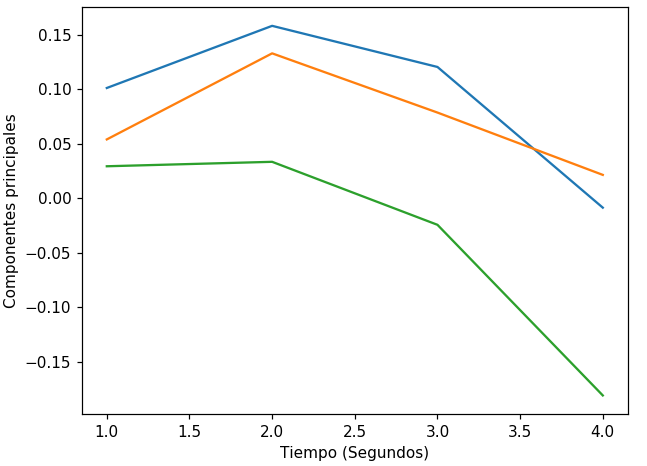
\includegraphics[width=1.5in]{imagenes/Cap4/pca3-4}}&\adj{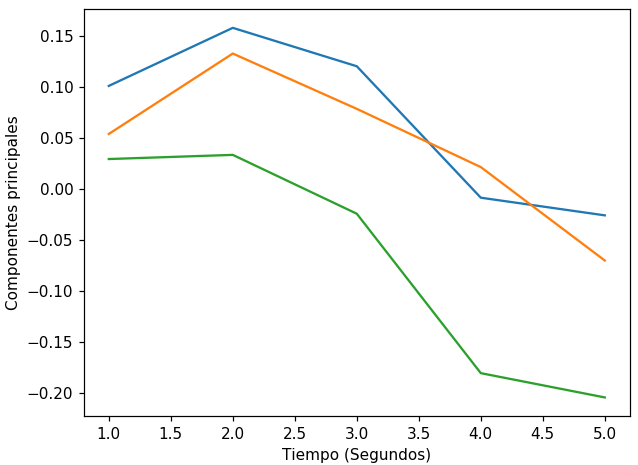
\includegraphics[width=1.5in]{imagenes/Cap4/pca3-5}} \\ \hline
4                                                                               & \adj{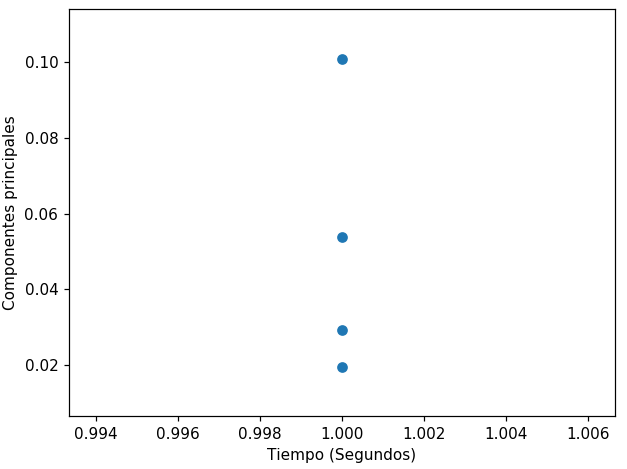
\includegraphics[width=1.5in]{imagenes/Cap4/pca4-1}} &\adj{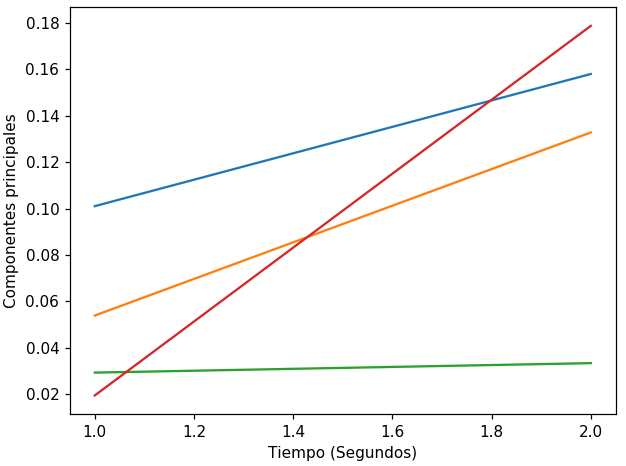
\includegraphics[width=1.5in]{imagenes/Cap4/pca4-2}}&\adj{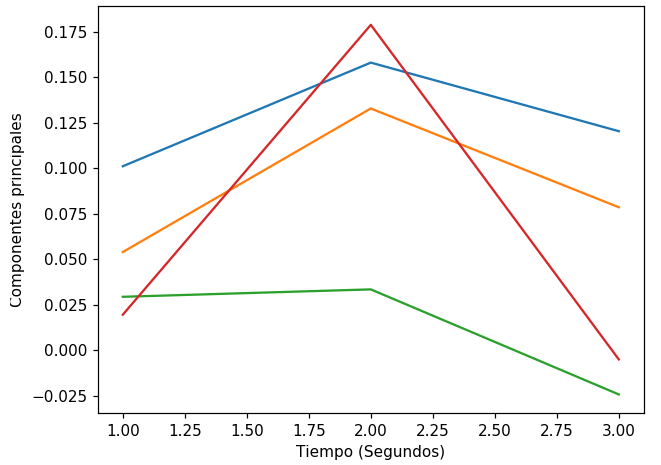
\includegraphics[width=1.5in]{imagenes/Cap4/pca4-3}}&\adj{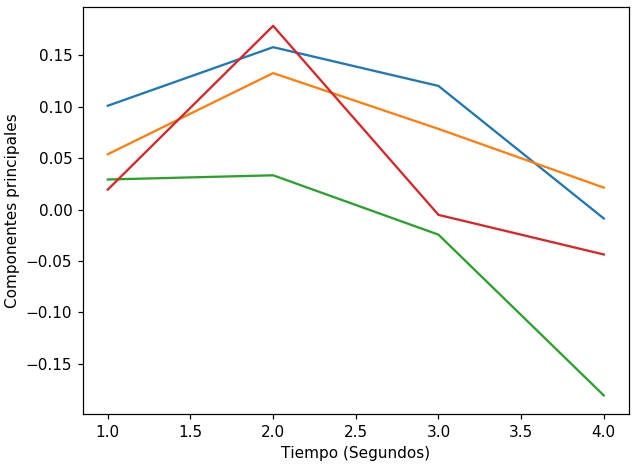
\includegraphics[width=1.5in]{imagenes/Cap4/pca4-4}}&\adj{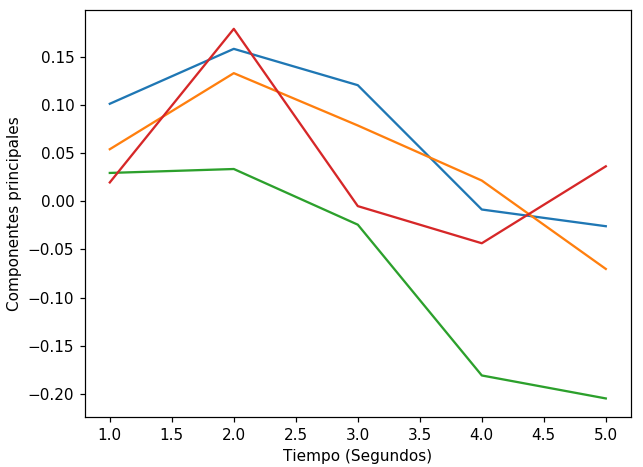
\includegraphics[width=1.5in]{imagenes/Cap4/pca4-5}} \\ \hline
\end{tabular}
\caption{Tabla con diferentes tama\~{n}os de series de tiempo para 3 y 4 componentes principales.}
  \label{table:series-de-tiempo}
\end{table}
\end{landscape}

\pagestyle{thesis}

Una vez definido como se tratar\'{a} el conjunto de datos se puede proceder con la siguiente fase (modelo ajustado al comportamiento normal).

\section{Modelo del comportamiento normal}

Esta etapa es una de las partes m\'{a}s importantes de \'{e}ste trabajo debido a que el rendimiendo del modelo de detecci\'{o}n de anomal\'{i}as depende en gran parte a la capacidad  de esta etapa
 
 

\section{Autoencoders para la detecci\'{o}n de anomal\'{i}as}

El m\'{e}todo tradicional de detecci\'{o}n de anomal\'{i}as basada en autoencoder es una forma de aprendizaje semi supervisado, se basa principalmente en el error de reconstrucci\'{o}n, considerando como anomal\'{i}as aquellas muestras que presentan un alto error de reconstrucci\'{o}n. En la fase de entrenamiento, solo se usan datos normales para entrenar el autoencoder, con el objetivo de minimizar el error de reconstrucci\'{o}n, de modo que el autoencoder pueda reconocer las caracter\'{i}sticas de los datos normales. En la fase de prueba, el autoencoder entrenado podr'{a} reconstruir datos normales con peque\~{n}os errores de reconstrucci\'{o}n, pero fallar\'{a}n con datos an\'{o}malos que el autoencoder no ha encontrado antes y, por lo tanto, tienen errores de reconstrucci\'{o}n relativamente m\'{a}s altos en comparaci\'{o}n a los datos normales. Por lo tanto, al comparar si el puntaje de reconstrucci\'{o}n de una anomal\'{i}a est\'{a} por encima de un umbral predefinido, el autoencoder determinar si los datos presentados para la prueba son an\'{o}malos \cite{47}.

\begin{equation}
C(z) = \left\lbrace
\begin{array}{ll}
\textup{si } S_{z}\leq \textup{threshold} & \textup{Normal}\\
\textup{en otro caso } & \textup{Anormal}
\end{array}
\right.
\end{equation}



\vspace{5mm} %5mm vertical space
